\chapter{Implemented languages}
\label{chap:implemented-langs}

As DortDB aims to support any query language, we have implemented three initial languages, one for each major data model. None of the languages was implemented completely. Given that DortDB does not aim to support data definition and manipulation (at least initially), the languages were trimmed to their data selection subset. Additionally, most of the typing and schema validation features were removed, as they couple the language too tightly with the underlying data representation.

\section{SQL}

SQL (standing for Structured Query Language) is a relational query language based on relational algebra and relational calculus. It became an ISO standard in 1987; the latest version of the standard was published in 2023\cite{sql_iso_2023}. The language operates in terms of tables (relations). Each table has a schema, which consists of a name and a set of attributes. Tables contain rows (tuples), whose values are called columns and correspond to the schema attributes. Important SQL operations include joins of relations and data aggregation.

The DortDB SQL language is based on the PostgreSQL SQL flavor\footnote{\url{https://www.postgresql.org/}}. It also includes several of the PostgreSQL JSON access operators.

\subsection{Notable features}

PostgreSQL includes several features that are not usual in other SQL flavors. Among them belong the following:

\subsubsection*{Lateral joins}

Lateral joins allow joining of correlated subqueries. In other words, it is possible for the joined subquery to refer to previous tables, and thus to be re-evaluated for different outer contexts.

\begin{minted}{sql}
SELECT t1.attr1, s.attr2 FROM t1
JOIN LATERAL (
  SELECT t2.attr2 FROM t2
  -- the WHERE clause refers to the outer context
  -- the subquery is reevaluated for each t1 row
  WHERE t2.attr3 + t1.attr4 > t1.attr5
) AS s
\end{minted}

\subsubsection*{\texttt{DISTINCT ON}}

The \texttt{DISTINCT} modifier filters out duplicate values. PostgreSQL allows customizing this behavior.

\begin{minted}{sql}
SELECT DISTINCT ON (attr1, attr2 % 10) attr1, attr2, attr3
FROM t1
\end{minted}

\subsubsection*{Complex aggregate calls}

The arguments of aggregate calls such as \texttt{count} or \texttt{sum} may be filtered or sorted.

\begin{minted}{sql}
SELECT
  count(DISTINCT attr1) AS distinct_count,
  count(attr1) FILTER (WHERE attr1 % 2 = 0) AS even_count,
  collect(attr1 ORDER BY attr1) AS ordered_array
FROM t1
\end{minted}

\subsection{Schema of data sources}
\label{subsec:sql-schema-data-sources}

SQL expects tables to have a clearly defined schema. This enables users to write queries that would otherwise be ambiguous.

\begin{minted}{sql}
-- which tables are a, b, or c from?
SELECT a, b, c
-- what columns are used in the natural join?
FROM t1 NATURAL JOIN t2
\end{minted}

DortDB data sources are, however, schemaless by design. Therefore, the allowed SQL queries face some restrictions. It must be clear from which tables specific columns originate. Non-qualified column names are only allowed when there is only a single, non-joined data source. Natural joins are disabled. All \texttt{FROM} clause subqueries must have an alias. Selecting all attributes using asterisk \texttt{*} is also disabled, although in theory it should be possible. When an attribute should not be interpreted as belonging to the current table, it should be prefixed by the \texttt{nonlocal} schema. This becomes relevant later, when inserting SQL subqueries into languages that do not prefix identifiers, such as Cypher.

\begin{minted}{sql}
-- t1.attr1
SELECT attr1 FROM t1
-- t2.attr2, t2.attr3, t1.attr1
WHERE (SELECT attr2 FROM t1 WHERE attr3 < nonlocal.attr1)
\end{minted}

To optimize the query plan later, some knowledge about the schema of the data sources and of the individual logical plan operators is necessary. Therefore, all of the referenced attributes must be paired with their data sources to infer their schema. This process happens once the logical plan is built and all of the used attributes are known.

\subsection{Not implemented features}

Besides data types, there are features that are not currently part of the DortDB SQL. The parser recognizes them, but they have not yet been implemented. The functionality will be added sometime in the future. This includes window functions, special \texttt{GROUP BY} features such as \texttt{ROLLUP}, or (possibly recursive) common table expressions.

\section{XQuery}

XQuery\footnote{\url{https://www.w3.org/TR/2014/REC-xquery-30-20140408}} is a functional programming language designed for querying structured and semi-structured XML data. It contains a superset of XPath\footnote{\url{https://www.w3.org/TR/xpath-31/}}, an expression language for querying XML. XPath operates in terms of sequences of values. Sequences cannot be nested; a sequence of sequences is interpreted as if it were flattened. Conversely, the values can be interpreted as sequences with one element. Null values are treated as empty sequences. XQuery adds SQL-like FLWOR expressions, named after some of the available clauses: For, Let, Where, Order by, and Return. Within FLWOR expressions, data is streamed as sequences of named tuples of values, but a FLWOR expression may return only sequences of opaque items. XQuery cannot accept or produce tuples.

\begin{minted}{xquery}
for $x in $source/foo (: $source/foo is an XPath expression :)
let $y := $x/bar (: $y is a sequence :)
(: data is passed between clauses
   as tuples with attributes x and y :)
return $y (: the result of the FLWOR is a flattened sequence :)
\end{minted}

Aggregation in XQuery is done by passing a sequence into a function. For example, summing numbers from 1 to 10 can be done like so:

\mint{xquery}{sum(1 to 10)}

XPath defines an expression's static and dynamic context. The static context consists of information available during the expression's static analysis and contains information such as statically known namespaces or in-scope variables. The dynamic context contains the current context item (referenced by a single dot or by the special variable \texttt{\$fs:dot}), the current context position (referenced by the function \texttt{fn:position()} or by the special variable \texttt{\$fs:position}), and the current context size (referenced by the function \texttt{fn:last()} or by the special variable \texttt{\$fs:last}).

\begin{minted}{xquery}
declare namespace foo = "http://example.org";
(: the static context now includes the foo namespace :)

(5 to 10)[
  (:
  the predicate can access the current item (numbers from 5 to 10),
  the current position (numbers from 1 to 5),
  and the current context size (number 5)
  :)
  . mod 2 eq 1
]
(: the result is the sequence (5,7,9) :)
\end{minted}

DortDB XQuery is a subset of XQuery 3.0.

\subsection{Not implemented features}

The DortDB XQuery implementation does not include any typing except \texttt{cast} expressions. This means that the following is not (and is not ever planned to be) available:

\begin{itemize}
    \item \texttt{as} keyword
    \item \texttt{typeswitch} expressions
    \item \texttt{instance of} expressions
    \item \texttt{treat} expressions
    \item \texttt{instance of} expressions
    \item \texttt{castable} expressions
    \item \texttt{validate} expressions
    \item any function types except \texttt{function(*)} 
    \item function references containing arity information (\texttt{fnname\#arity})
\end{itemize}

The following is also not implemented, but may be added in the future:

\begin{itemize}
    \item \texttt{try catch} expressions
    \item pragma expressions
    \item \texttt{window} FLWOR clause
    \item inline functions
    \item \texttt{\%private} and \texttt{\%public} modifiers
    \item any module prolog except namespace definition
\end{itemize}

\section{Cypher}

Cypher is a declarative graph query language developed for the Neo4j database\footnote{\url{https://neo4j.com/docs/cypher-manual/25/introduction/}}. The DortDB Cypher language is based on openCypher, which is an open source specification of Cypher. Since the release of GQL (Graph Query Language) by ISO\footnote{\url{https://www.iso.org/standard/76120.html}} in April 2024, the aim of the openCypher project is to converge towards GQL and ease the transition of graph databases towards the ISO standard.

Cypher operates on labeled property graphs, a graph data model in which both nodes and relationships may contain properties. Furthermore, nodes may have zero or more labels, while each relationship has exactly one type. Relationships are always directed.

\begin{figure}[ht!]
  \centering
  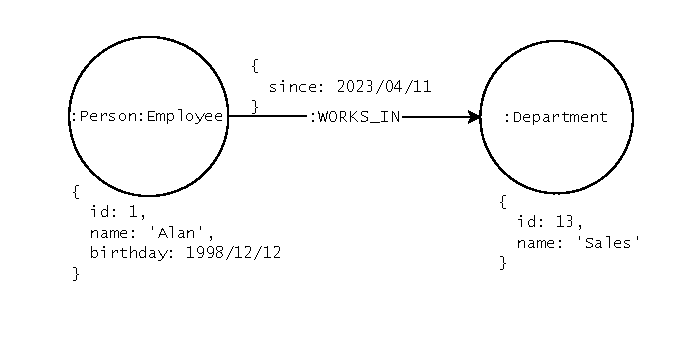
\includegraphics[width=0.7\textwidth]{img/lpg.pdf}
  \caption{Labeled property graph}
  \label{fig:lpg}
\end{figure}

\pagebreak

Cypher provides a visual way of matching patterns and relationships using ASCII art. It is possible to match recursive paths. A matched path cannot contain duplicate relationships, but each node may be visited multiple times.

\begin{minted}{cypher}
    §\textcolor{teal}{\texttt{\textup{//} \textit{match each neighbor of Alan, regardless of direction}}}§
    §\textcolor{teal}{\texttt{\textup{//} \textit{the neighbors will be stored in the 'neighbor' variable}}}§
    MATCH (:Person {name: "Alan"})-[]-(neighbor)

    §\textcolor{teal}{\texttt{\textup{//} \textit{match Alan's friends of friends, up to three hops far,}}}§
    §\textcolor{teal}{\texttt{\textup{//} \textit{and then find their employers}}}§
    §\textcolor{teal}{\texttt{\textup{//} \textit{the p variable will contain a list of relationships}}}§
    MATCH ({name: "Alan"})-[p:KNOWS *1..3]->(foaf)
      <-[:EMPLOYS]-(employer)

    §\textcolor{teal}{\texttt{\textup{//} \textit{the recursive path may match patterns like}}}§
    §\textcolor{teal}{\texttt{\textup{//} \textit{(alan)->(x)->(alan)->(y)}}}§
    §\textcolor{teal}{\texttt{\textup{//} \textit{but it cannot match the same relationship twice}}}§
    §\textcolor{teal}{\texttt{\textup{//} \textit{(alan)->(x)->(alan)->(x)}}}§
\end{minted}

It is then possible to process the matched values similarly to SQL.

\begin{minted}{cypher}
    MATCH (x)-[]->(y)
    WHERE y.age < 15
    RETURN x.name, y.age
    ORDER BY x.name
    SKIP 3
\end{minted}

\subsection{Differences between DortDB and openCypher}

The DortDB Cypher language is parsed with an LALR(1) parser, which is not powerful enough for the original openCypher grammar, as it has only a limited lookahead. The grammar contains constructs that would be ambiguous during parsing. We have, therefore, decided to always parse certain patterns a certain way, even though it means that some otherwise valid queries will fail.

\subsubsection*{Node patterns or parenthesized expressions}

If the input can be interpreted as either the start of a node pattern or a parenthesized expression, the parser will always choose the node pattern.

\begin{itemize}
    \item \texttt{(a)} is a node pattern
    \item \texttt{(a:Label)} is a node pattern
    \item \texttt{(\{prop: value})\} is a node pattern
    \item \texttt{(\$param)} is a node pattern
\end{itemize}

Because of this, \texttt{(a:Label = true)} will cause a parsing error, because it is already considered a node pattern, even though it would be a valid expression in the original grammar, checking whether the \texttt{a} variable has the \texttt{Label} label. The same goes for \texttt{({prop: value}.prop)}. More complex parenthesized expressions starting with a variable or a parameter are not affected, for example, \texttt{(\$param = true)} or \texttt{(a + a)} are valid expressions.

This should not cause any issues, as it is always possible to interpret the input as expressions by removing the parentheses. The label check expression \texttt{a:Label} has the highest precedence, so parentheses would not do anything anyway, and the rest are simply parentheses around atomic expressions.

\subsubsection*{Operators}

The following symbol combinations are considered part of relationship patterns and will not be interpreted as operators. If necessary, it is always possible to clarify the meaning by adding parentheses.

\begin{itemize}
    \item \texttt{<-[} (e.g., it will never be parsed as a comparison like \texttt{a < -[b]})
    \item \texttt{<--}
    \item \texttt{--}
    \item \texttt{-[}
\end{itemize}

\subsubsection*{List/pattern comprehension or list literals}

Cypher includes special syntax for list comprehension and pattern comprehension.

\begin{minted}[ignorelexererrors=true]{cypher}
RETURN [x IN range(0,10) WHERE x % 2 = 0 | x^3] AS result

MATCH (a:Person)
RETURN [(a)-[:KNOWS]->(b) WHERE b:Person | b.name] AS friends

MATCH (a {id: 1})
RETURN [path = (a)-[:KNOWS*]->(b) | size(path)] AS foafDistances
\end{minted}

If the input can be interpreted as either the start of a list/pattern comprehension or a list literal, the parser will always choose the list/pattern comprehension. More specifically, if the input starts with:

\begin{itemize}
    \item \texttt{[variable IN}
    \item \texttt{[variable = (pattern)}
\end{itemize}

Then it is no longer possible to interpret it as a list literal (even though in the original grammar, \texttt{[variable IN list1, variable IN list2]} would be a valid list literal containing two booleans).

\subsubsection*{Reserved words}

In addition to the regular reserved words, the following words need to be escaped before they can be used as identifiers.

\begin{itemize}
    \item \texttt{COUNT}
    \item \texttt{ANY}
    \item \texttt{NONE}
    \item \texttt{SINGLE}
\end{itemize}